% !TEX root = ../diary-book.tex

\section{令和6年12月21日 シャワー測定頻度の推定}

\subsection{一次宇宙線到来頻度の推定（続き）}
2024-12-21 17:05:37

12月18日に引き続きシミュレーションを行っている。

1 - 100 TeVについて検出効率と到来頻度を見る。


\begin{figure}
   \begin{minipage}[t]{0.48\linewidth}
      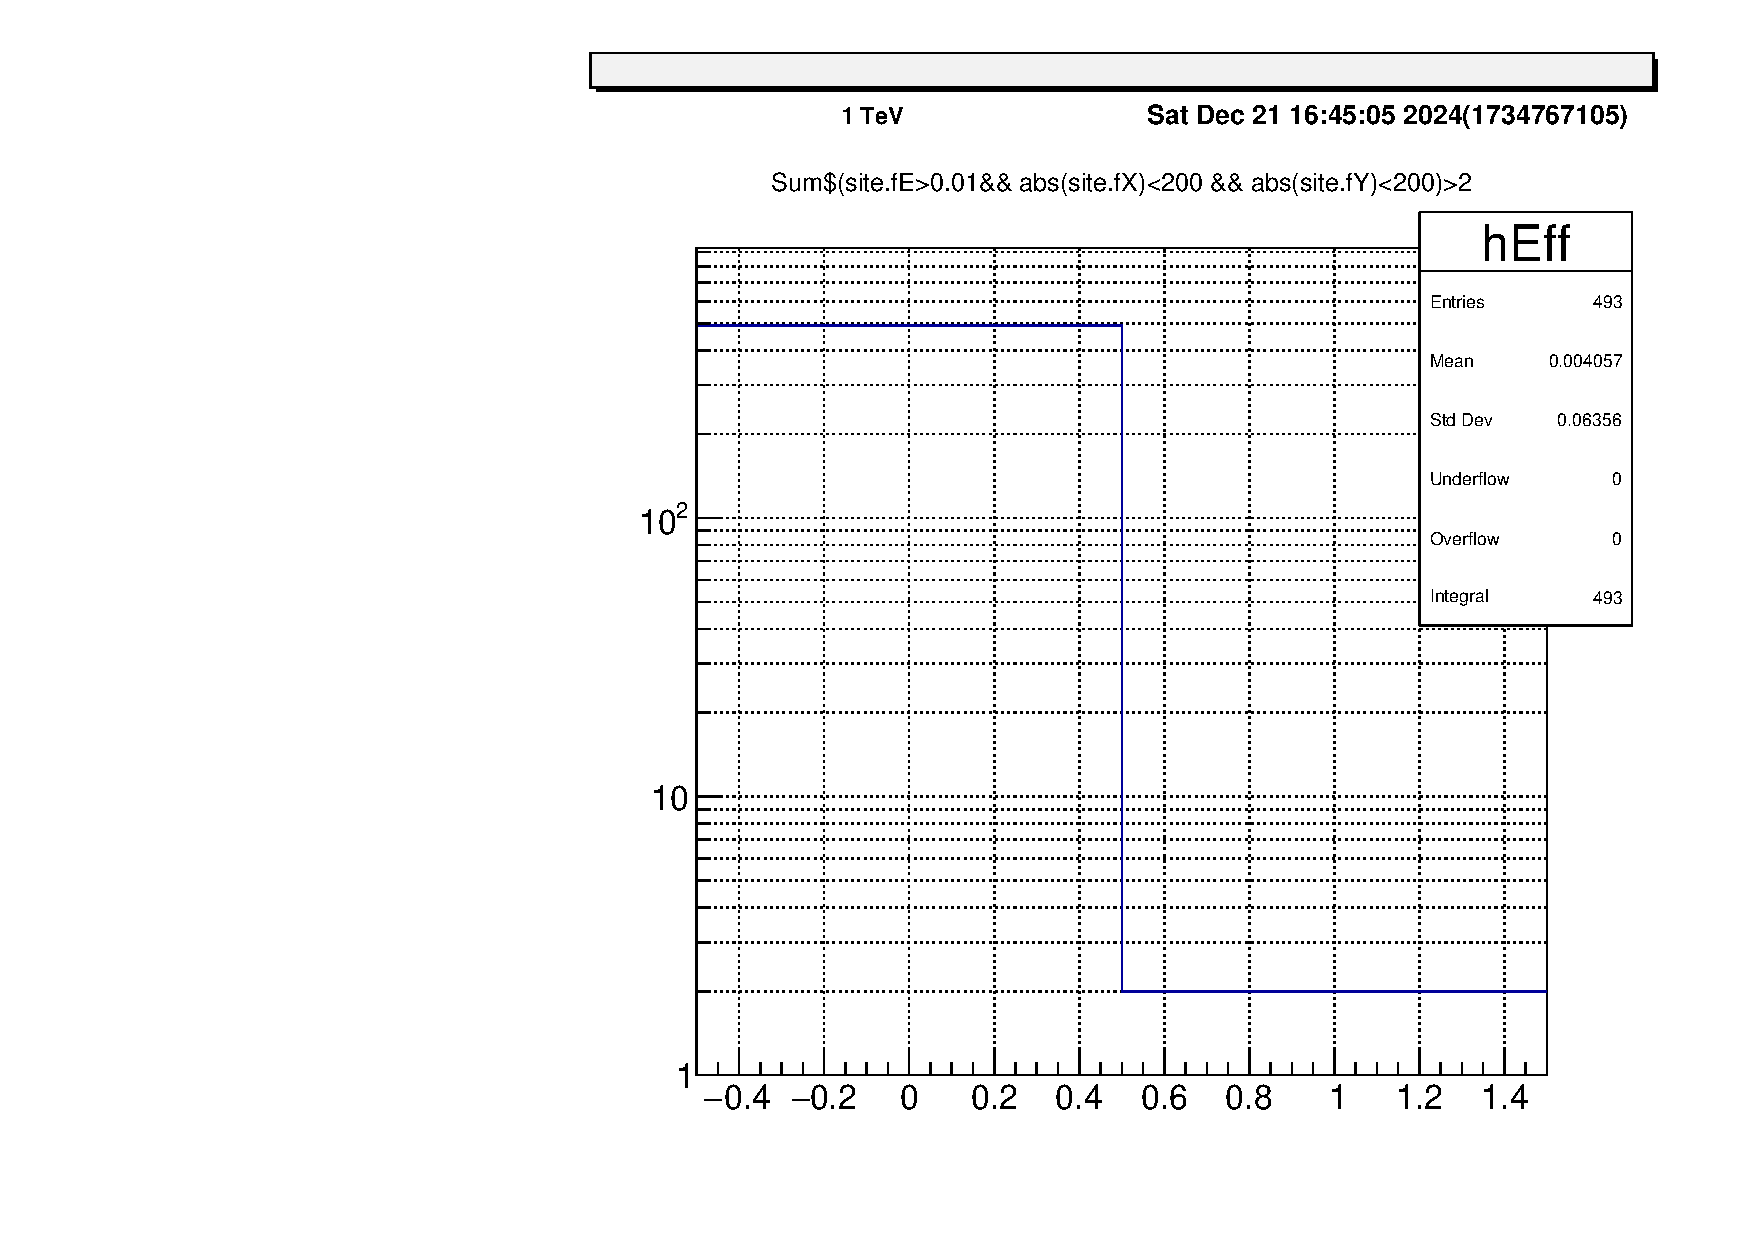
\includegraphics[width=.95\linewidth]{../../figs/ata03/figs/20241221/1734767105.pdf} % 1 TeV
      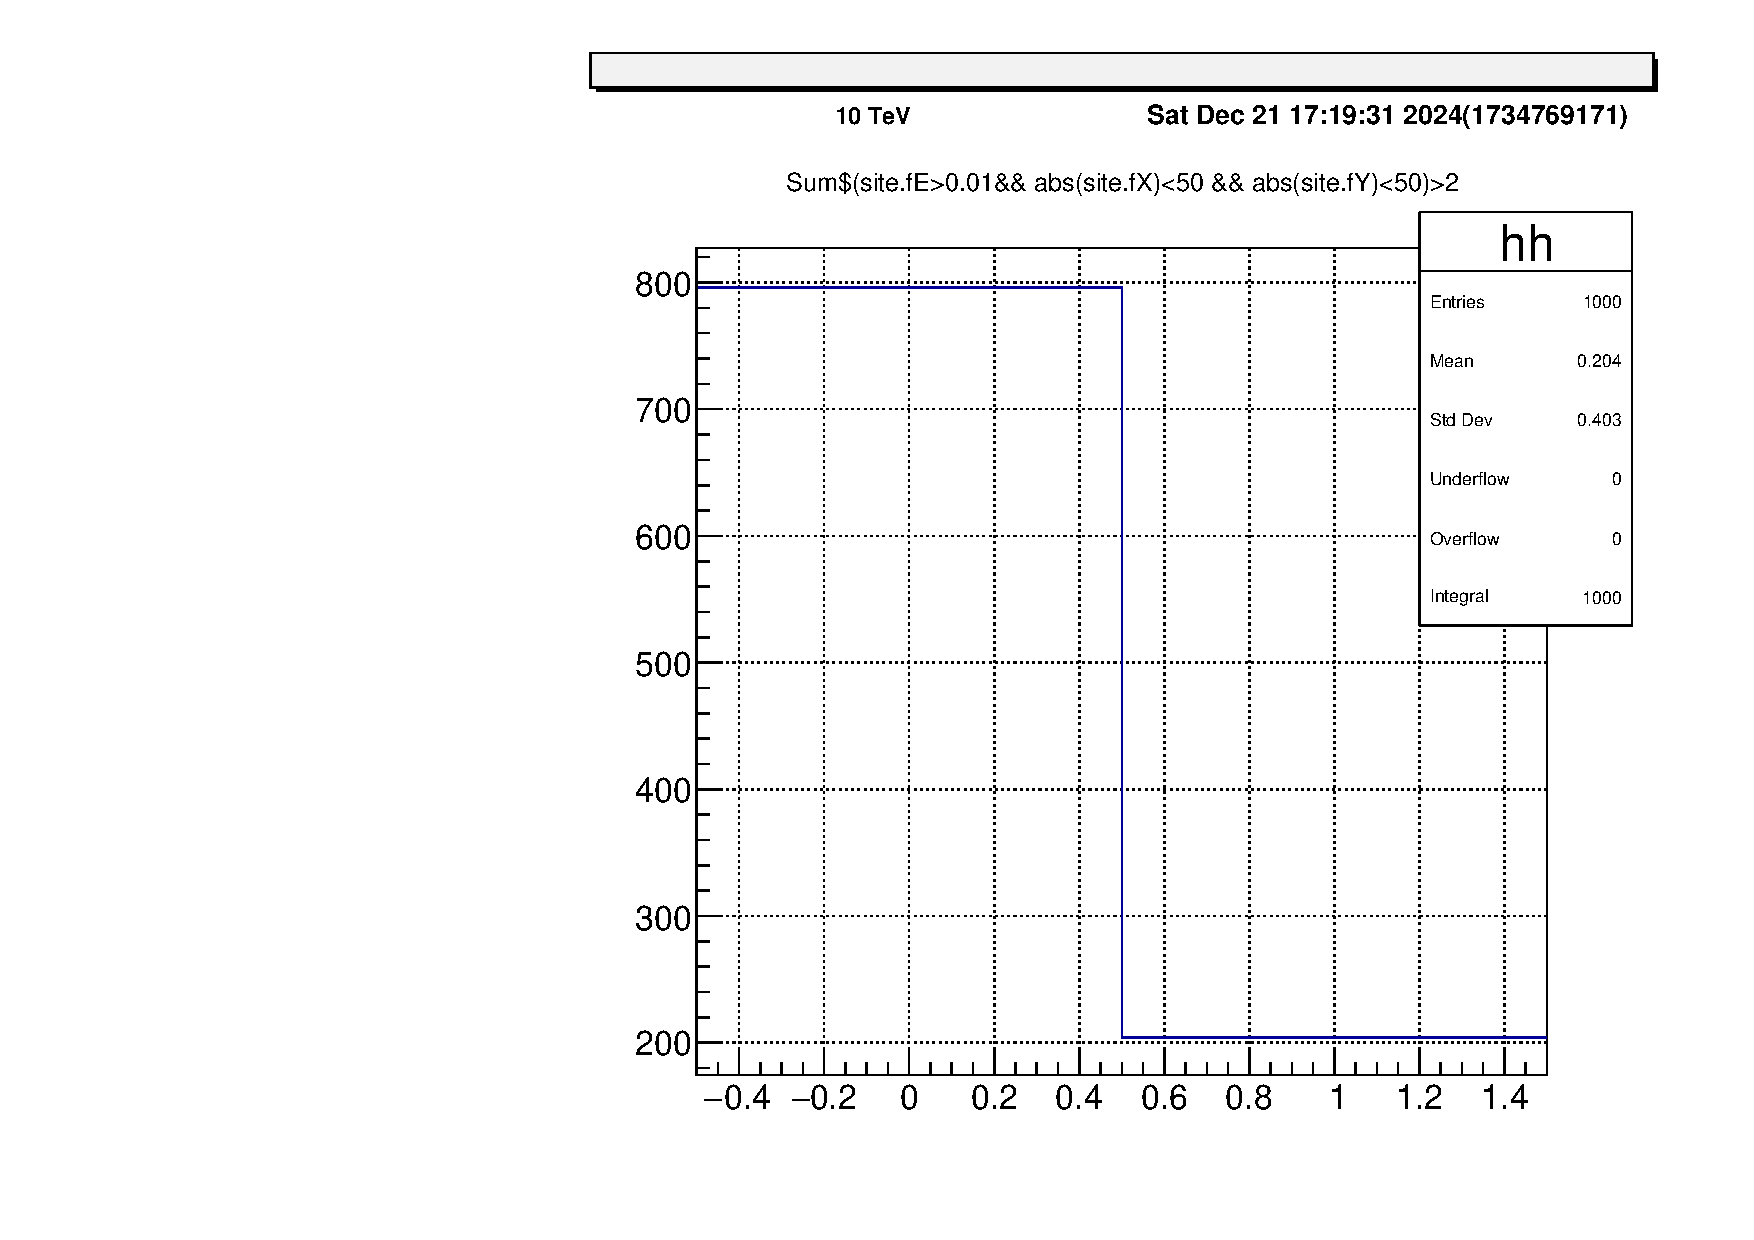
\includegraphics[width=.95\linewidth]{../../figs/ata03/figs/20241221/1734769171.pdf} % 10 TeV
      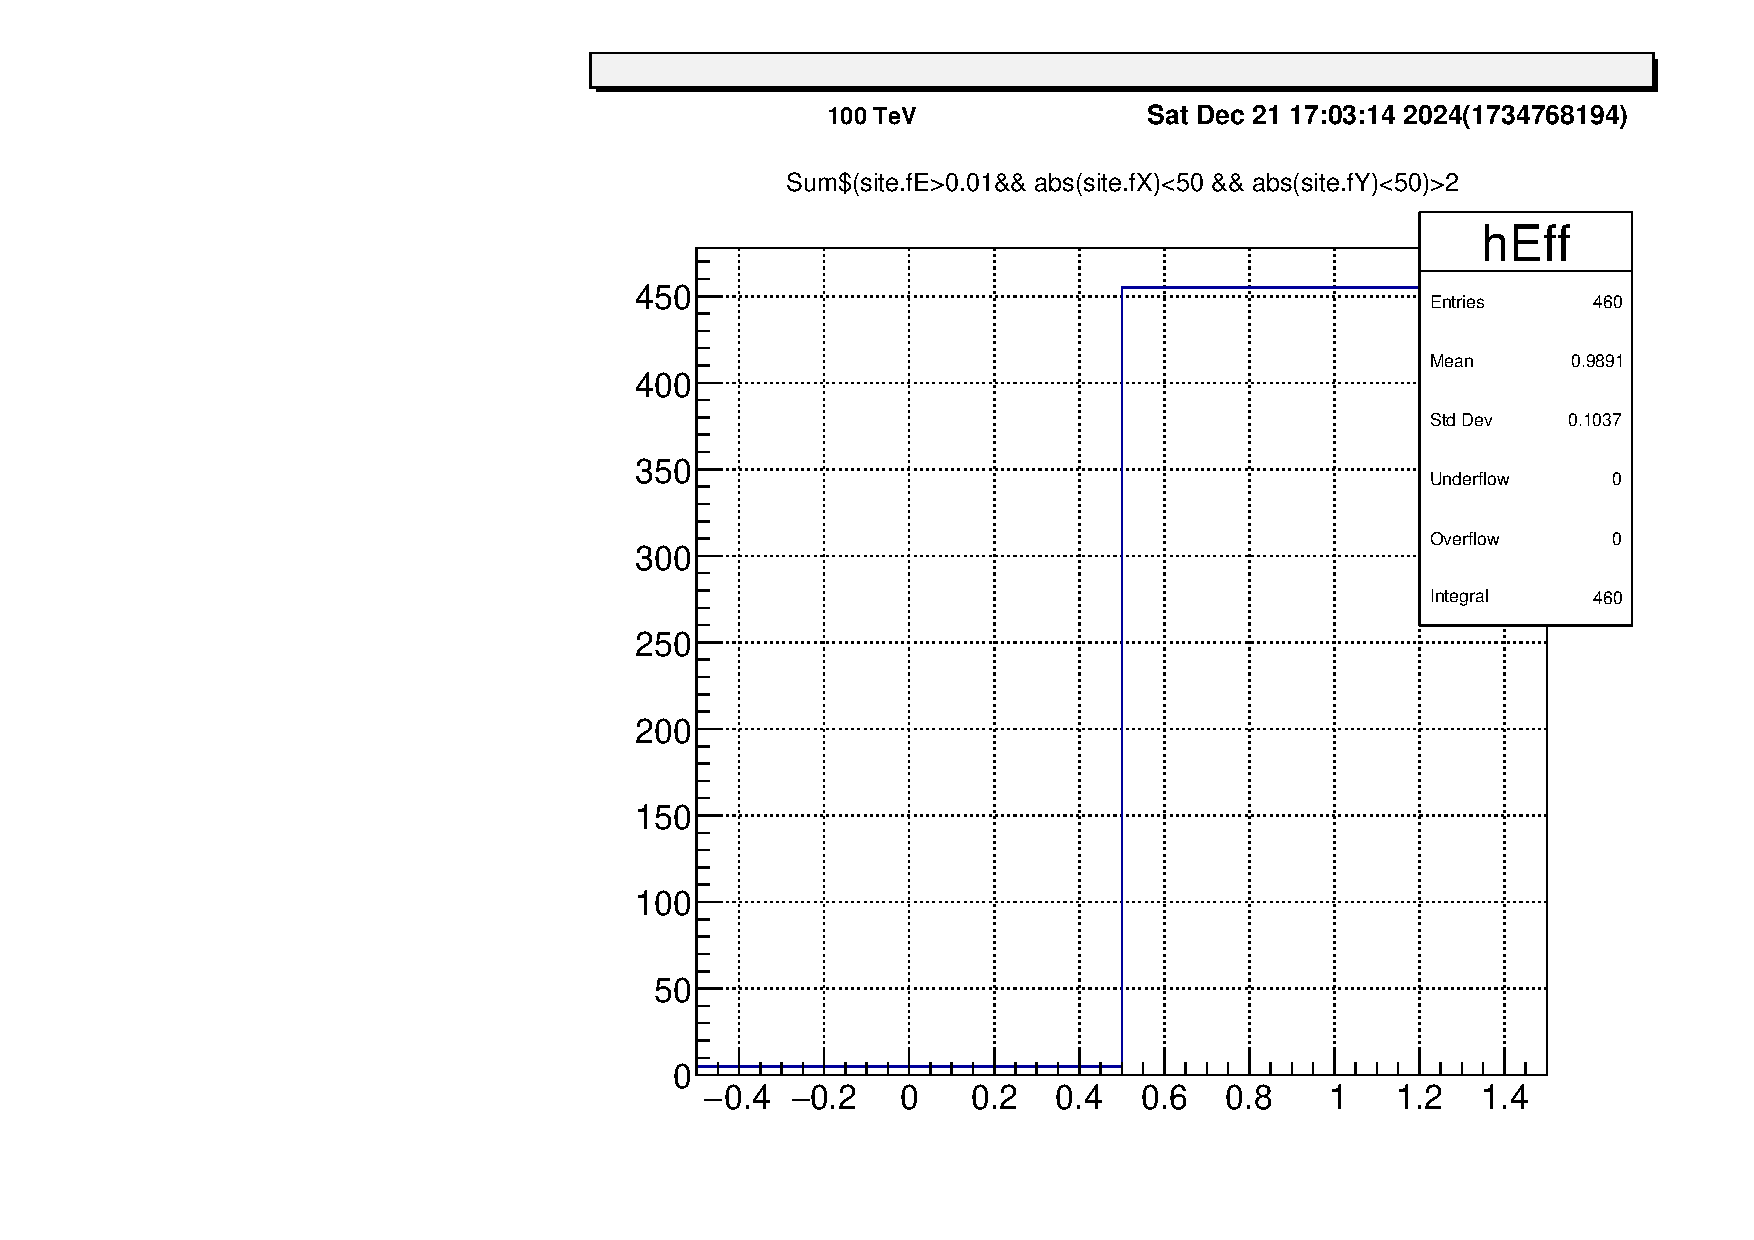
\includegraphics[width=.95\linewidth]{../../figs/ata03/figs/20241221/1734768194.pdf} % 100 TeV
   \end{minipage}
   \begin{minipage}[t]{0.48\linewidth}
      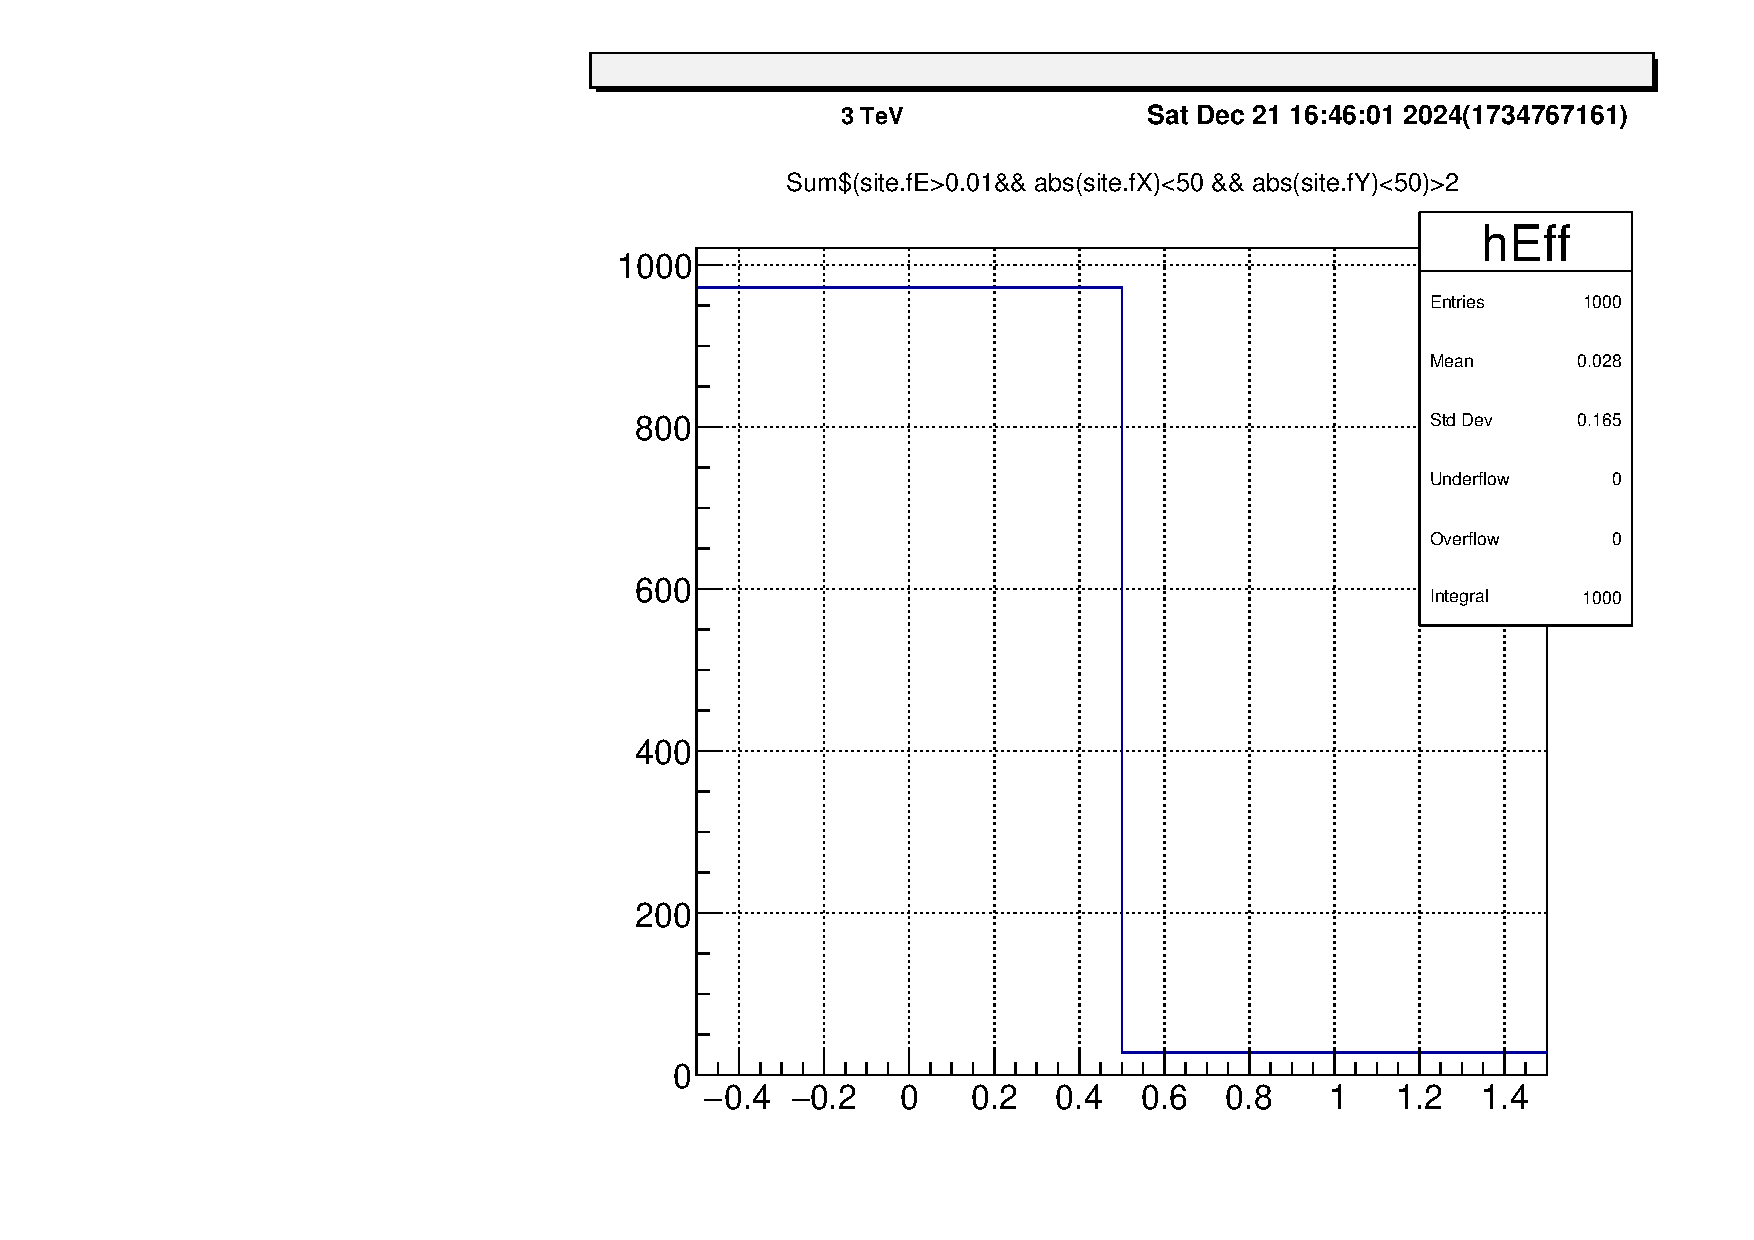
\includegraphics[width=.95\linewidth]{../../figs/ata03/figs/20241221/1734767161.pdf} % 3 TeV
      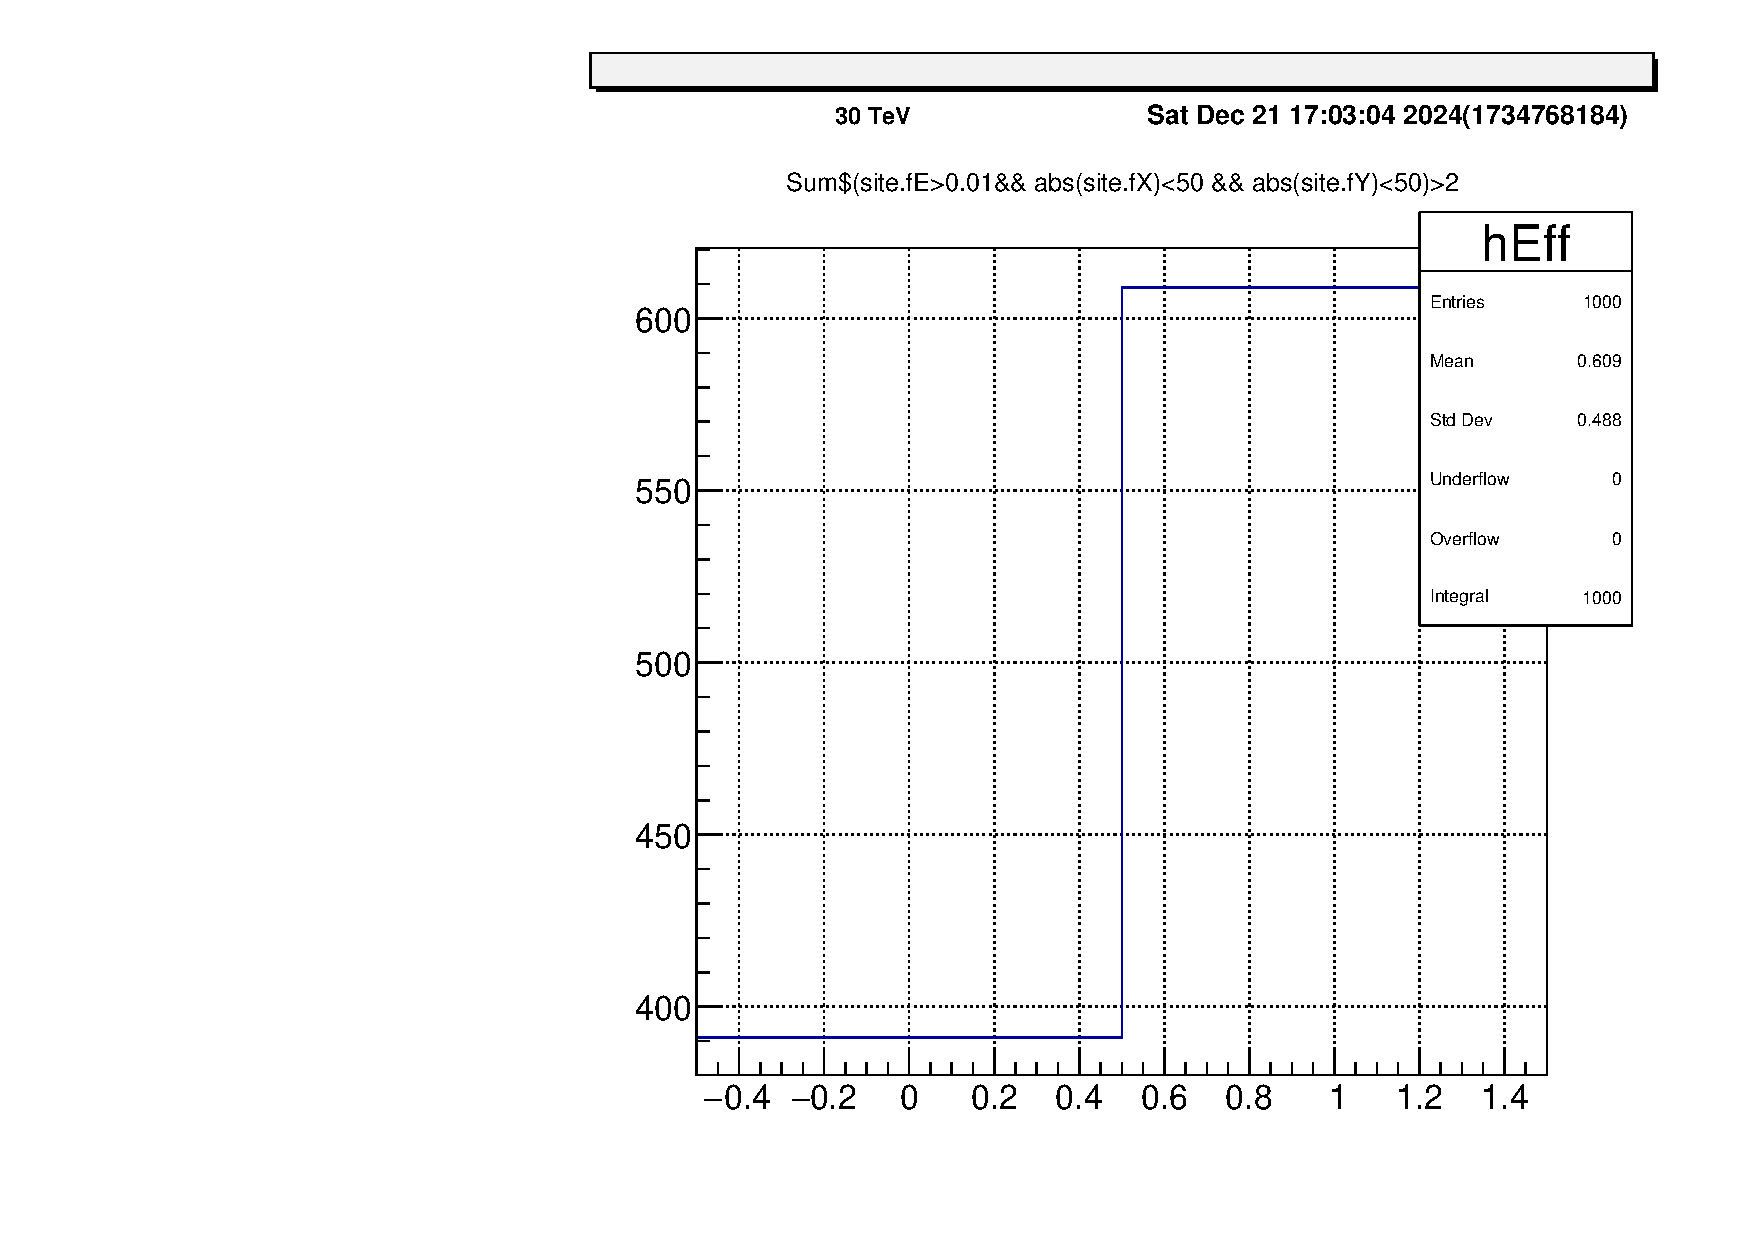
\includegraphics[width=.95\linewidth]{../../figs/ata03/figs/20241221/1734768184.pdf} % 30 TeV
   \end{minipage}
\end{figure}




\begin{table}[H]
   \centering
   \caption{シャワー同定頻度についての見積もりを行った。これらの積分値であるのでシャワー同定頻度は100~m四方の領域で毎秒1個程度であることがわかる。ミューオンがコインシデンスするかどうかはまた別の話。。。うーむ。到来頻度の立体角は $\pi/4$として計算してある。}
   \begin{tabular}[H]{cSSS}
      \hline
      \hline 
      一次宇宙線のエネルギー & {シャワー測定効率} & {到来頻度} & {シャワー同定頻度} \\
      (TeV) & &  {個/$10^4$~m$^2$/s} & {個/$10^4$~m$^2$/s} \\
      \hline
      1 & 0.004057 & 110.48 & 0.44821736\\
      3 & 0.028 & 6.856  & 0.191968 \\
      10 & 0.204 & 0.9958 & 0.2031432 \\
      30 & 0.609 & 0.0618 & 0.0376362 \\
      100 & 0.989 & 0.00987 & 0.00976143 \\
      \hline
      \hline
   \end{tabular}
\end{table}